\documentclass{article}
\usepackage[UTF8]{ctex}
\usepackage[T1]{fontenc}
\usepackage[utf8]{inputenc}
\usepackage{latexsym}
\usepackage{amsmath}
\usepackage{siunitx}
\usepackage{float}
\usepackage{xcolor}
\usepackage{listings}
\usepackage{graphicx}
\lstset{
    basicstyle = \ttfamily,
    keywordstyle = \bfseries,
    linewidth = \linewidth,
    xleftmargin=.2\textwidth,
    xrightmargin=.2\textwidth,
    numbers = left,
    numberstyle = \textcircled,
    frame = none,
}
\title{Homework 2}
\author{PB17000297 罗晏宸}
\date{March 20 2020}

\begin{document}
\maketitle

\section{}
使用以下代码段(假定 R3 的初值为 R2+396):

\begin{lstlisting}[language={[x86masm]Assembler}]
Loop:   LD      R1, 0(R2);
        DADDI   R1, R1, #1;
        SD      R1, 0, (R2);
        DADDI   R2, R2, #4;
        DSUB    R4, R3, R2;
        BNEZ    R4, Loop;
\end{lstlisting}
\subparagraph{a} 列出上述代码中的所有数据相关,需写出数据相关类型,并记录寄存器,源指令和目标指令。例如,从指令①到指令②存在对于寄存器 R1 的 RAW 相关。
\subparagraph{b} 给出这一指令序列对于 5 级 RISC 流水线的时序,该流水线没有设置任何旁路定向路径(Bypass or Forwarding),但假定在同一时钟周期中的寄存器读取与写入通过该寄存器堆进行“转发”,且分支是通过冲刷流水线来处理的。如果所有存储器引用耗时一个周期,这一循环的执行需要多少个周期?
\subparagraph{c} 给出这一指令序列对于拥有完整旁路定向路径的 5 级 RISC 流水线的时序。如果所有存储器引用耗时一个周期,且在处理分支时采用预测转移失败策略,这一循环的执行需要多少个周期?
\subparagraph{d} 给出这一指令序列对于拥有完整旁路定向路径的 5 级 RISC 流水线的时序。如果所有存储器引用耗时一个周期,且在处理分支时采用预测转移成功策略,这一循环的执行需要多少个周期?

\paragraph{解}
\subparagraph{a}
\subparagraph{b}
\subparagraph{c}
\subparagraph{d}

\section{}
有一条静态多功能流水线由 5 段组成,加法用 1,3,4,5 段,乘法用 1,2,5 段,第三段的时间为$2\Delta t$ ,其余各段时间均为$\Delta t$ ,而且流水线的输出可以直接返回输入端或暂存于相应的流水寄存器中。现要在该流水线上计算$\displaystyle \prod_{i = 1}^4(A_i + B_i)$,画出其时空图,并计算其吞吐率、加速比和效率。
\begin{figure}[h]
    \centering
    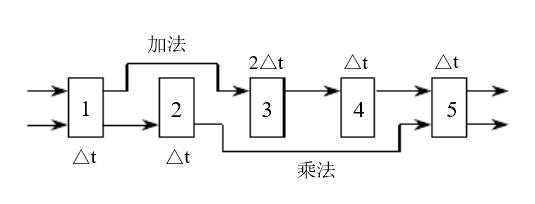
\includegraphics[width = 270pt]{2.jpg}
\end{figure}
\paragraph{解}

\section{}
假定原机器是一个 5 级流水线,其时钟周期为 \SI{1}{\nano\second}。第二种机器为 12 级流水线,时钟周期为 \SI{0.6}{\nano\second}。由于数据相关,5 级流水线每 5 条指令经历一次 stall,而 12级流水线每 8 条指令经历三次 stall。此外,分支占全部指令的 20\%,两台机器的预测错误率都是 5\%。
\subparagraph{a} 仅考虑数据相关,12 级流水线相对于 5 级流水线的加速比为多少?
\subparagraph{b} 在考虑分支预测错误而导致 stall 的情况下,如果第一台机器的分支预测错误的额外代价为 2 个周期,而第二台机器为 5 个周期,则每种机器的 CPI 为多少?

\paragraph{解}

\end{document}